\documentclass{article}
\usepackage{graphicx}
\usepackage{caption}
\graphicspath{ {./images/} }
 
\begin{document}
\paragraph{nslookup}
\begin{itemize}
  \item\begin{enumerate}
    \item Run nslookup to obtain the IP address of a Web Server in Asia, What is the ip address of that Server?
      \begin{itemize}
        \item IP Address: 14.139.45.149 \par
        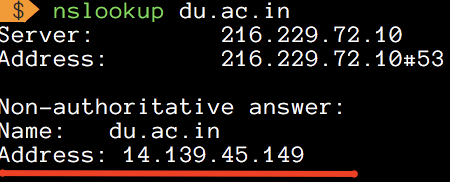
\includegraphics[scale=0.8]{images/nslook1.png}
      \end{itemize}
    \item Run nslookup to determine the authoritative DNS servers for a university in Europe
        \begin{itemize}
          \item 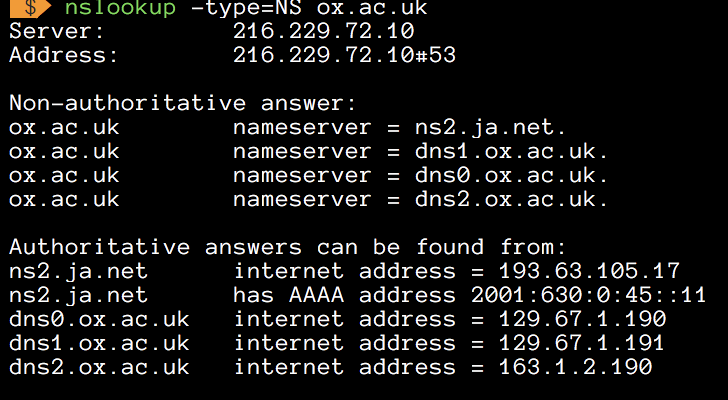
\includegraphics[scale=0.6]{images/nslookup2.png}
        \end{itemize}

    \item Run nslookup so that one of the DNS servers obtained in question 2 is queried for the mail servers for yahoo! mail.  What is its IP address?
        \begin{itemize}
          \item 
        \end{itemize}
  \end{enumerate}
\end{itemize}

\paragraph{Tracing DNS with wireshark}
\begin{itemize}
  \item\begin{enumerate}
    \item Locate the DNS query and response messages. Are they sent over UDP or TCP?
      \begin{itemize}
        \item The DNS query is being sent over UDP \par
        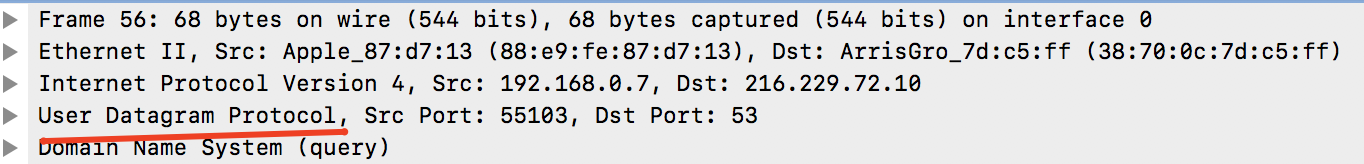
\includegraphics[scale=0.4]{images/DNS4.png}
      \end{itemize}
    \item What is the destination port for the DNS query message? What is the source port of DNS response message?
        \begin{itemize}
          \item Source Port: 55103
          \item Destination Port: 53\par
          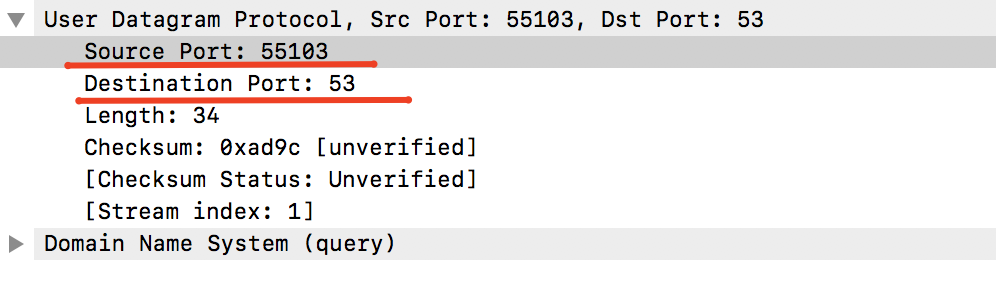
\includegraphics[scale=0.5]{images/DNS5.png}
        \end{itemize}
    \item To what ip address is the dns query message sent use ipconfig to deetermine the ip address of your local dns server. Are these two ip addresses the same?
        \begin{itemize}
          \item The Query is sent to 226.229.72.10, the addresses are the same\par
          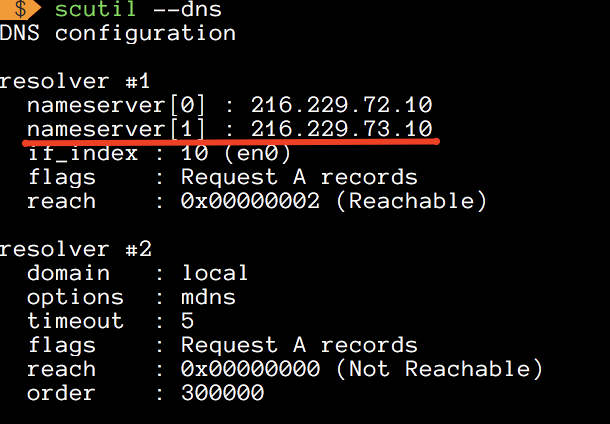
\includegraphics{images/DNS6.png}\par
          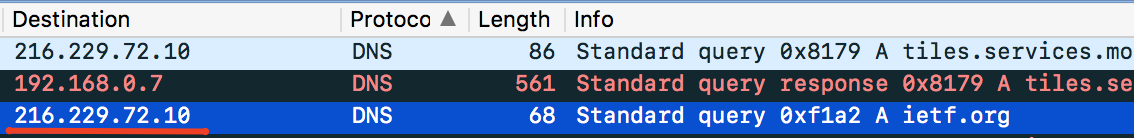
\includegraphics[scale=0.5]{images/DNS6b.png}
        \end{itemize}

    \item Examine the DNS query message.  What "Typee" of DNS query is it? Does the query message containy and "answers"?
    \begin{itemize}
      \item It is a standard Type A query and contains no "Answers"\par
      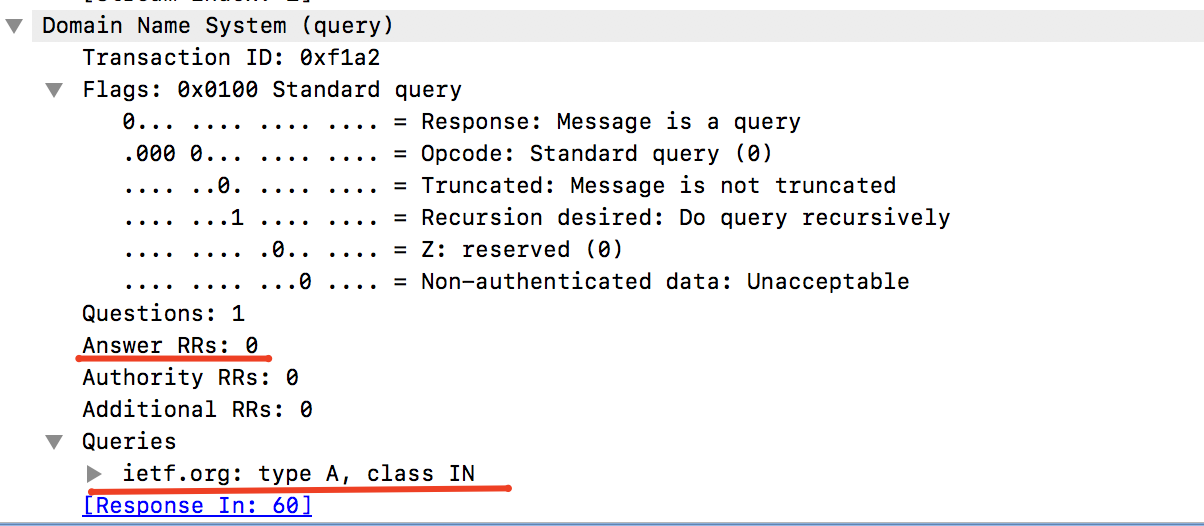
\includegraphics[scale=0.6]{images/DNS7.png}
    \end{itemize}  
    \item Examine the DNS response message.  How many "answers" are provided?  What do each of these answers contain?
    \begin{itemize}
      \item The DNS response contains one "answer" with all of the information on ietf.org that we requested, including the ip address\par
      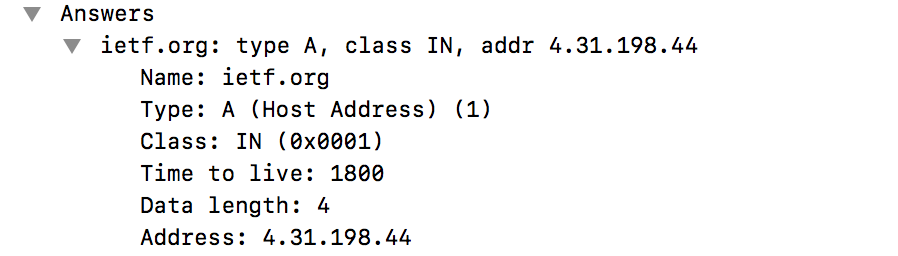
\includegraphics[scale=0.5]{images/DNS8.png}
    \end{itemize}

    \item Consider the subsequent TCP SYN packet sent by your host.  Does the destination IP address of the SYN packet correspond to any of the IP addresses provided in the DNS response message?
    \begin{itemize}
      \item Yes, the destination address of the TCP SYN packet matches the returned IP address of ietf.org that we requested in the previous step
      \item 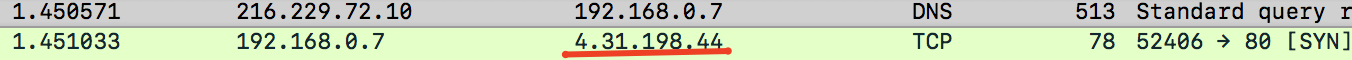
\includegraphics[scale=0.5]{images/DNS9.png}
    \end{itemize}

    \item What is the destination port for the DNS query message? What is the source port of the DNS response message?
    \begin{itemize}
      \item The Desination port for the DNS query is 53, the source port for the Response message is 53 aswell.
      \item 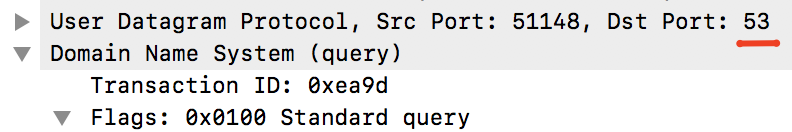
\includegraphics[scale=0.5]{images/DNS11a.png}
      \item 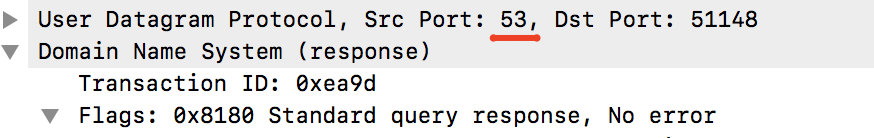
\includegraphics[scale=0.5]{images/DNS11b.png}
    \end{itemize}

    \item To what IP address is the DNS query meessage sent?  Is this the IP address of your deefault local DNS server?
    \begin{itemize}
      \item IP Address: 216.229.72.10, This is the ip address of my local dns server.\par
      \item 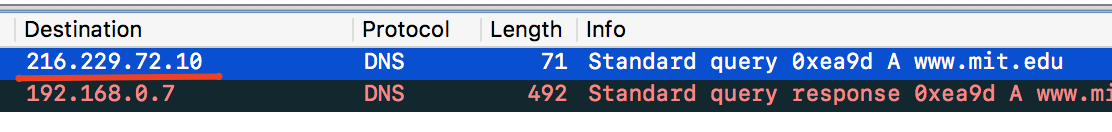
\includegraphics[scale=0.5]{images/DNS12.png}
    \end{itemize}

    \item Examine the DNS query mesesage.  What type of DNS query is it?  Dose the query message contain any "answers"?
    \begin{itemize}
      \item The Query is a standard Type A Query, it does not contain any answers
      \item 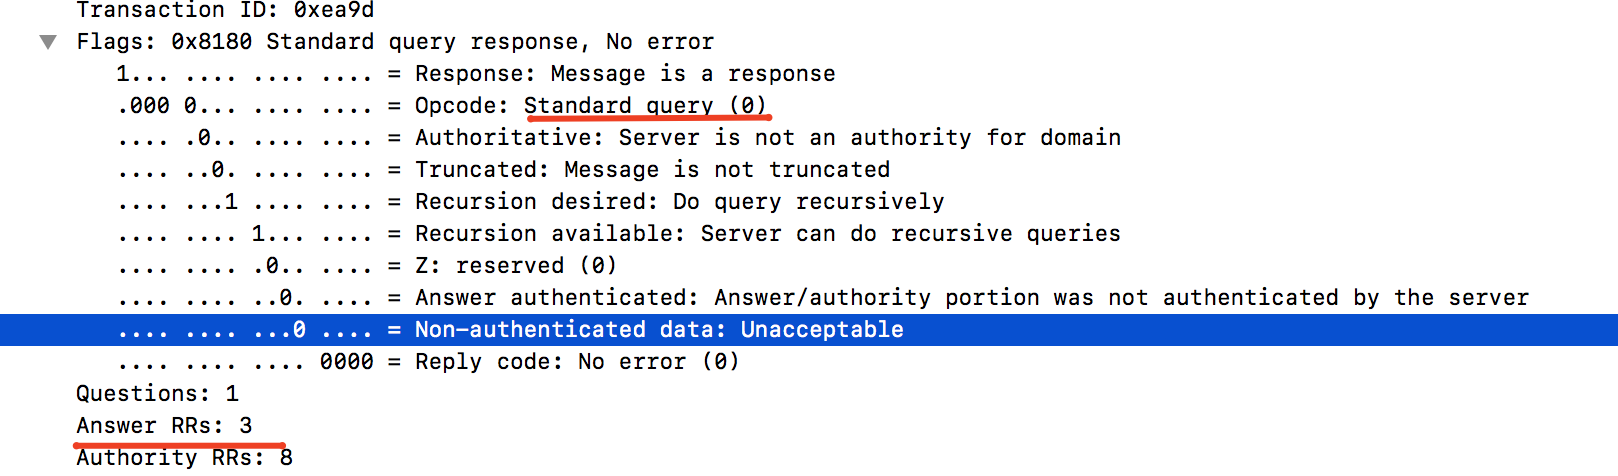
\includegraphics[scale=0.5]{images/DNS13.png}
    \end{itemize}

    \item examine the DNS response message.  How many answers are provided?  What do each of these answers contain?
      \begin{itemize}
        \item There are three Answers in the DNS response message.  There is one host address which corresponds to the ip address we request, and two CNAMES.
        \item 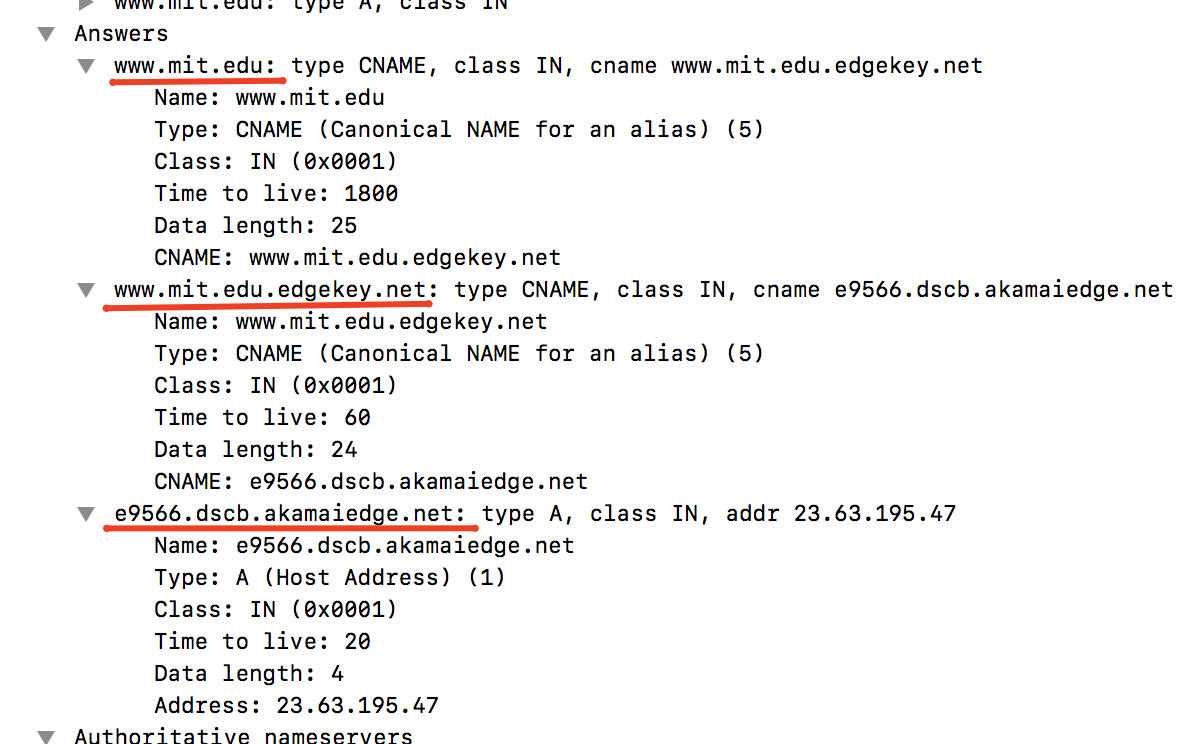
\includegraphics[scale=0.5]{images/DNS14.png}
      \end{itemize}


      \item To what IP address is the DNS query message sent? Is this the IP address of your default local DNS Server?
      \begin{itemize}
        \item 216.229.72.10, this is the ip address of my local DNS server.
        \item 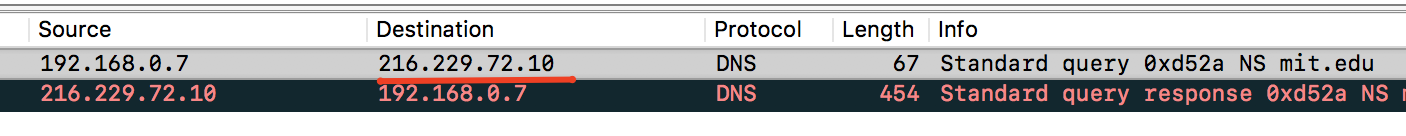
\includegraphics[scale=0.5]{images/DNS16.png}
      \end{itemize}
      \item Examine the DNS query message.  What "Type" of DNS query is it?  Does the query message contain any "answers"?
      \begin{itemize}
        \item The DNS Query is "NS" type and contains 8 answers.
        \item 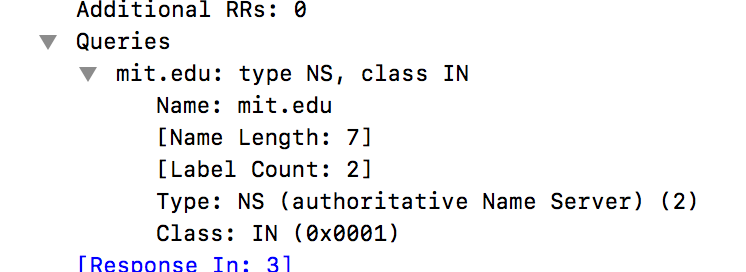
\includegraphics[scale=0.5]{images/DNS17.png}
      \end{itemize}
      \item Examine the DNS response message.  What MIT nameservers does the response message provide?  Does this reponse message also provide the IP addresses of the MIT nameservers?
      \begin{itemize}
        \item The response contains the Authoritative Nameservers, and does not provide IP addresses for the MIT nameservers.
        
      \end{itemize}
      \item Provide A Screenshot (Included to keep question numbers the same for easier grading)
      
      \item To what IP address is the DNS query message sent?  Is this the ip address of your default local DNS Server?  If not, what does the ip address correspond to?
      \begin{itemize}
        \item Two DNS queries are sent to 18.72.0.3, and One DNS query is sent to 216.229.72.10 which is my default dns server.  
        \item 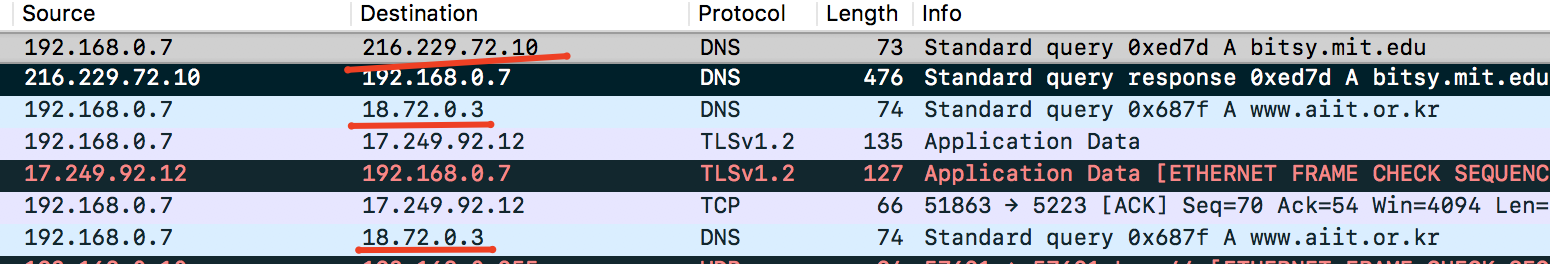
\includegraphics[scale=0.5]{images/DNS20.png}
      \end{itemize}
      \item Examine the DNS query message.  What "Type" of DNS query is it?  Does the query message contain any "answers"?
      \begin{itemize}
        \item All three DNS queries are standard Type A queries, and all three queries do not have answers.
        \item 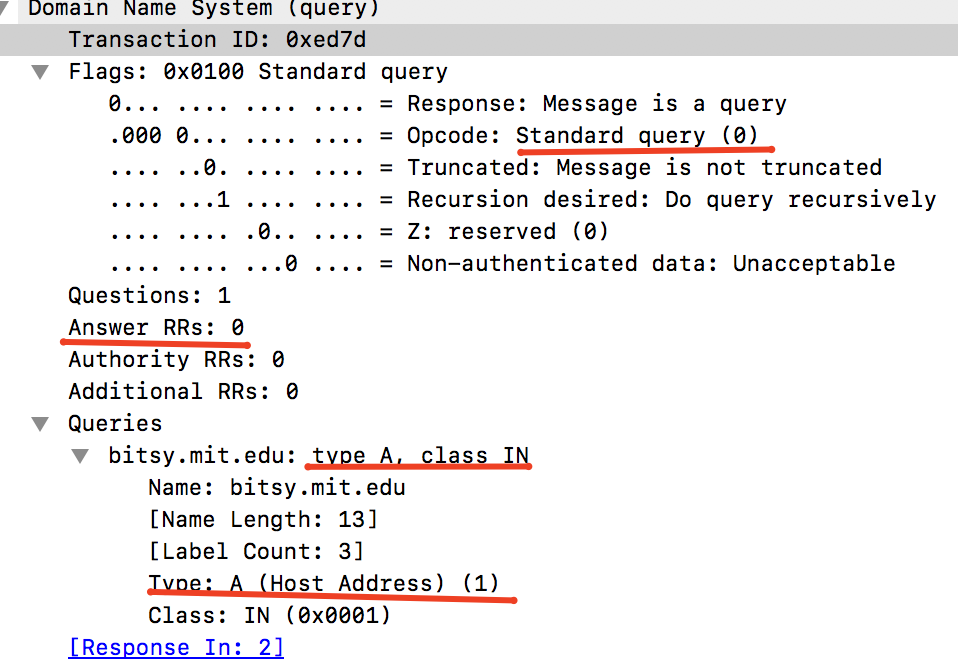
\includegraphics[scale=0.5]{images/DNS21.png}
      \end{itemize}
      \item Examine the DNs response message.  How many "answers" are priovided?  What does each of these answers contain?
      \begin{itemize}
        \item There is one Answer which conatins the ip of bitsy.mit.edu
        \item 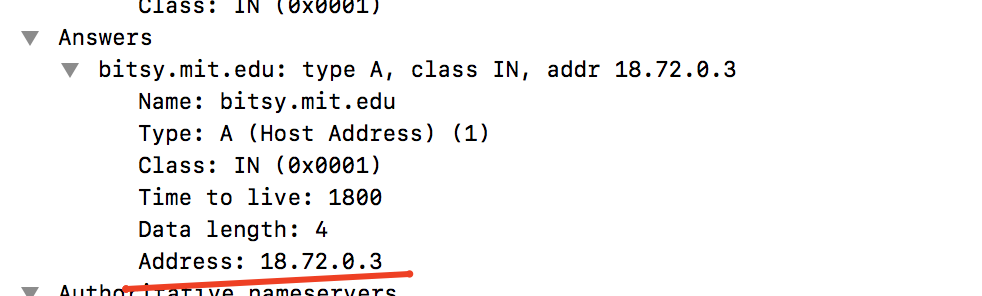
\includegraphics[scale=0.5]{images/DNS22.png}
      \end{itemize}
      \item Provide A Screenshot (Included to keep question numbers the same for easier grading)
  \end{enumerate}
\end{itemize}
\end{document}
